\capitulo{5}{Aspectos relevantes del desarrollo del proyecto}

\section{Desarrollo de la idea}

El proyecto inicial surgió a partir de un problema a la hora de repartir  el coste de un tique entre varios usuarios los cuales debían pagar el importe correspondiente por los artículos consumidos por cada uno, la idea era calcular esto de forma automática a partir de una aplicación en la que cada cliente introdujera el importe pagado y los artículos consumidos, los cuales se extraerían a partir de una imagen.

Esta idea se cambio por la siguiente propuesta, llevar a cabo una aplicación de gestión de gastos a partir de la cual, el usuario introduce una imagen de los productos consumidos y estos son almacenados de forma que, el usuario pueda consultar en cualquier momento en que se ha gastado su dinero.

\section{Tesseract como Libreria OCR \label{precisionTesseract}}

Para poder desarrollar el presente trabajo, se realizó una búsqueda preliminar de como poder llevar a cabo la extracción de los productos a partir de una imagen digital, para ello fue necesario la búsqueda de un OCR (\ref{ocr}) para poder realizar la  extracción del texto.
La herramienta propuesta por el tutor fue Tesseract, la cual permitía la obtención del texto a partir de un fichero de imagen, de forma gratuita y con una exactitud aceptable.

Se instaló y probó Tesseract en un entorno Linux, y se realizaron las siguientes pruebas a las imágenes \ref{fig:original1},\ref{fig:recortada1},\ref{fig:original2} y\ref{fig:recortada2}

\begin{itemize}
	\item Sin ninguna configuración con diccionario de caracteres Ingleses.
	\item Configuración en bloque con diccionario de caracteres Ingleses.
	\item Configuración en linea con diccionario de caracteres Ingleses.
	
	\item Configuración en palabra con diccionario de caracteres Ingleses.
	
	\item Sin ninguna configuración con diccionario de caracteres Español.
	\item Configuración en bloque con diccionario de caracteres Español.
	\item Configuración en linea con diccionario de caracteres Español.

\item Configuración en palabra con diccionario de caracteres Español.

\end{itemize}

\begin{figure}[ht]
		\centering
		\begin{minipage}[b]{0.45\linewidth}
			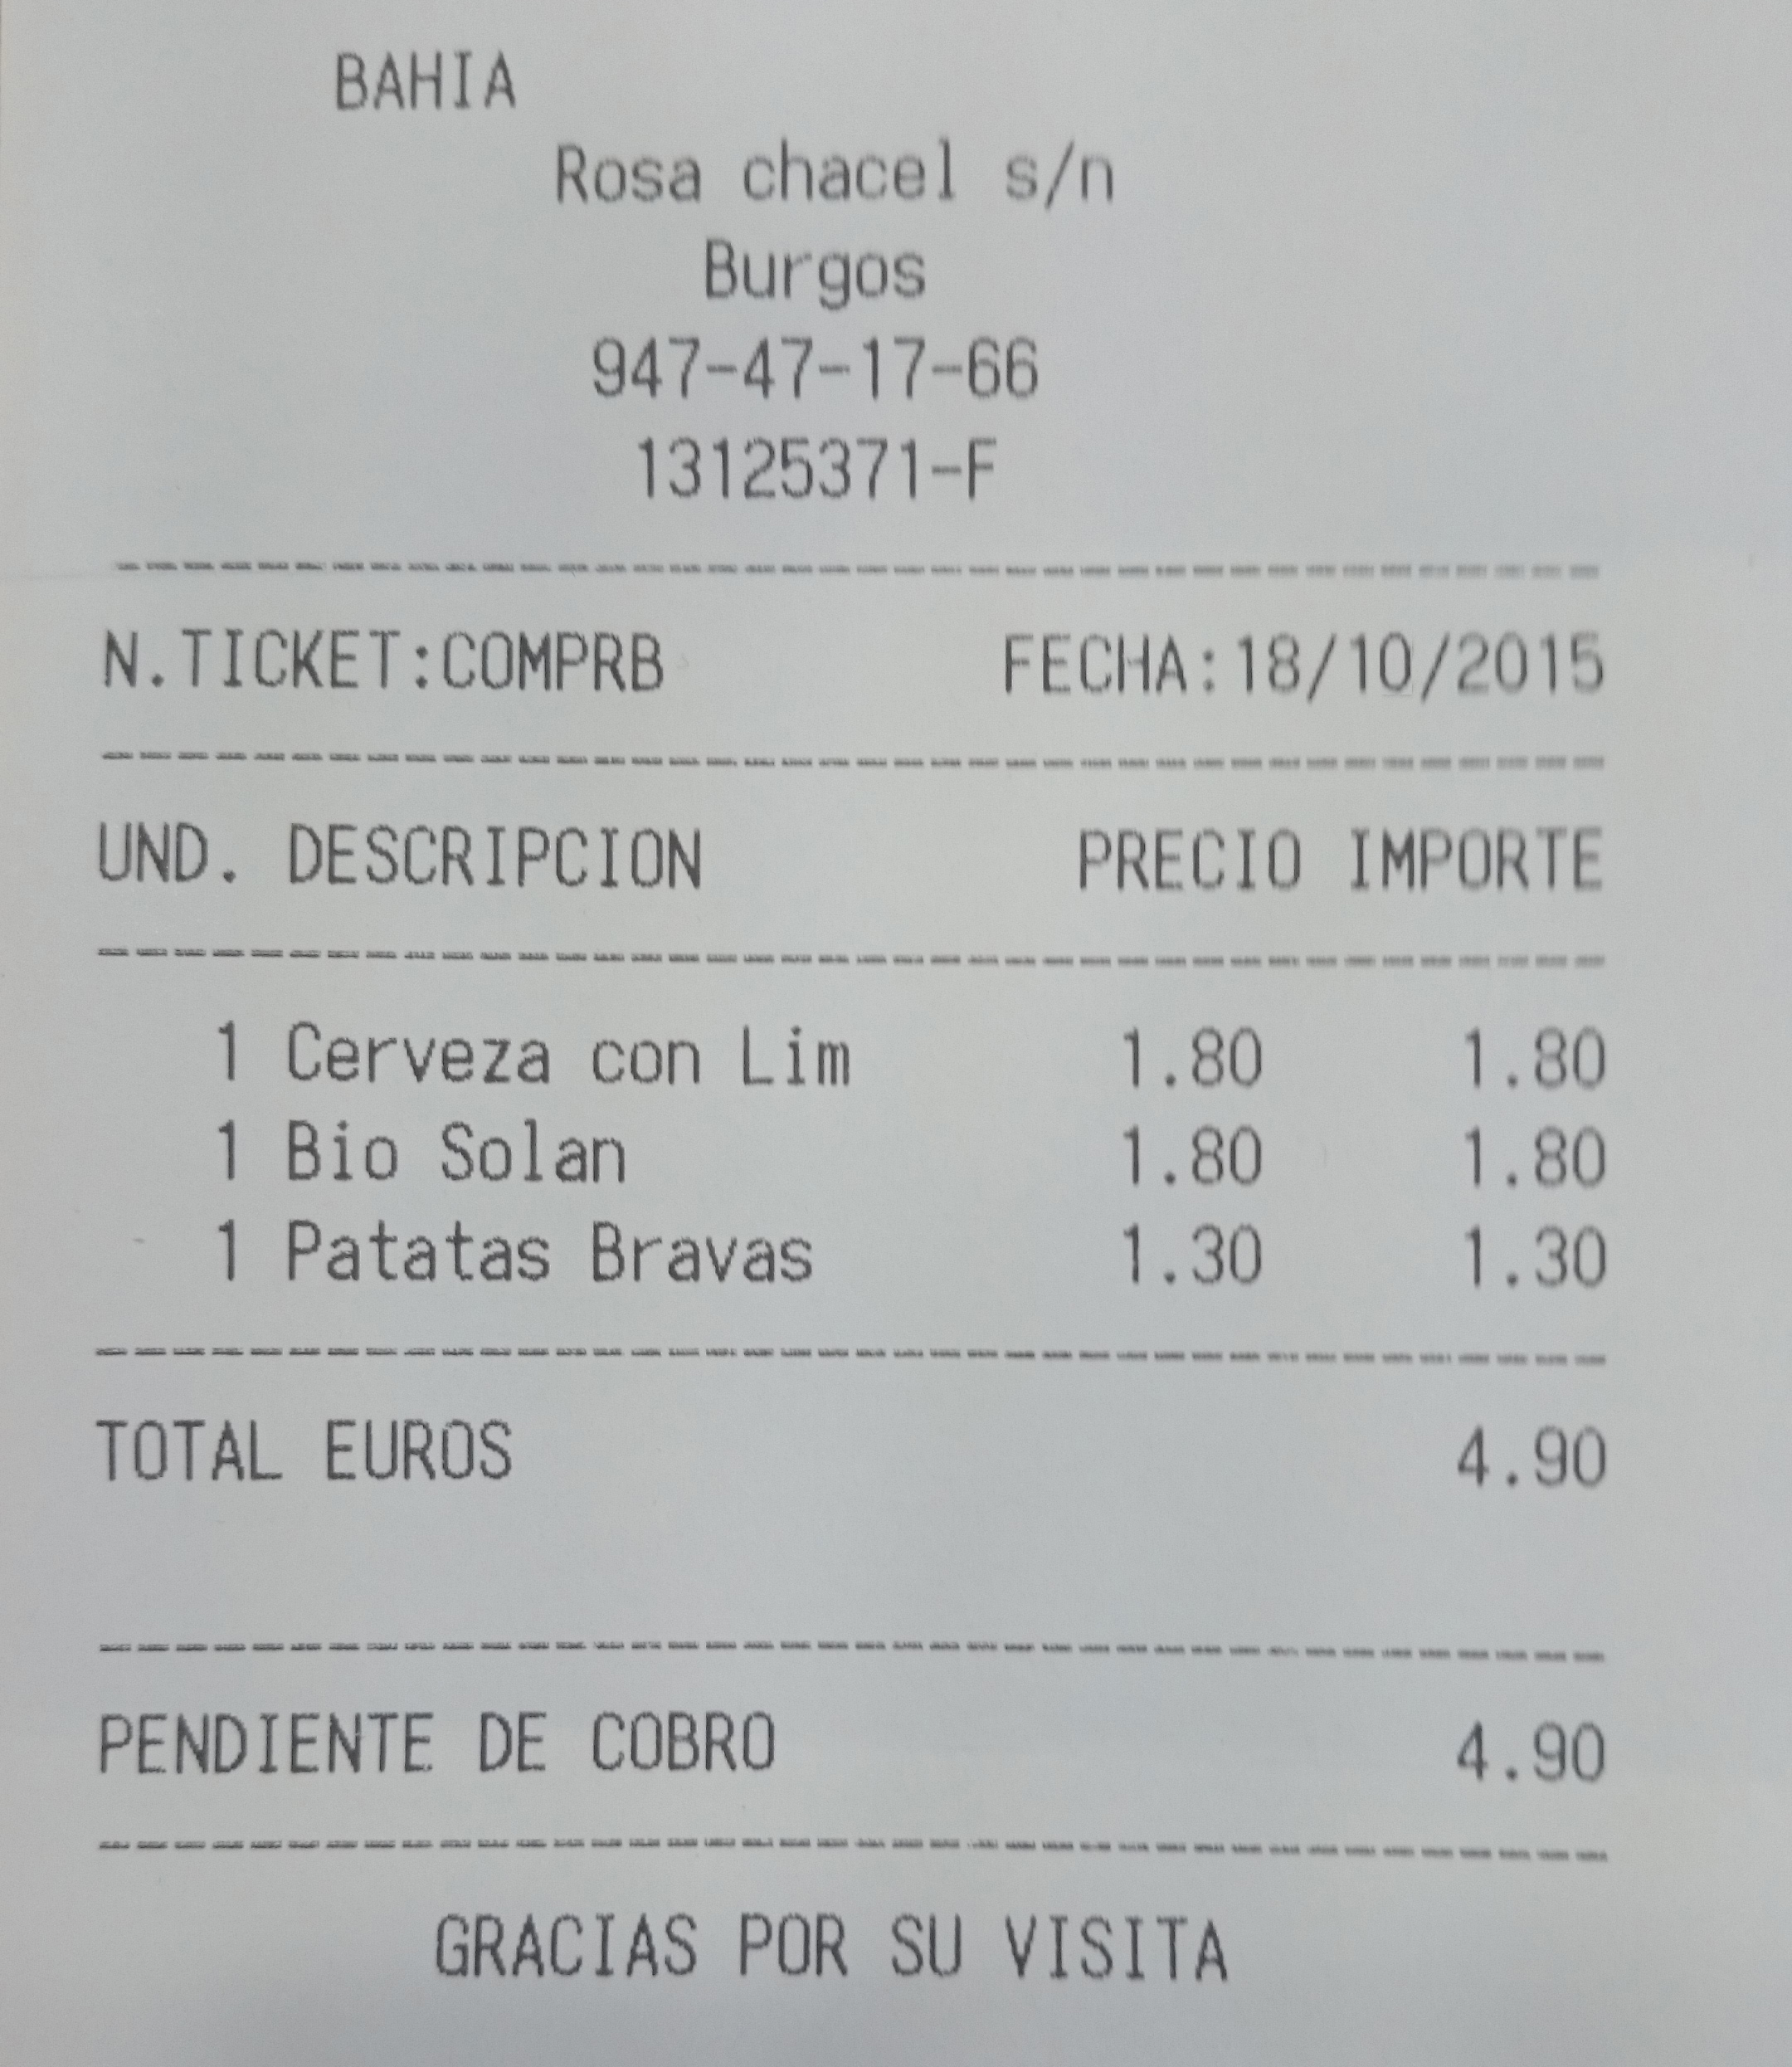
\includegraphics[width=\linewidth]{Original1.jpg}
			\caption{Imagen Original nº 1}
			\label{fig:original1}
	\end{minipage}
	\quad
	\begin{minipage}[b]{0.45\linewidth}
		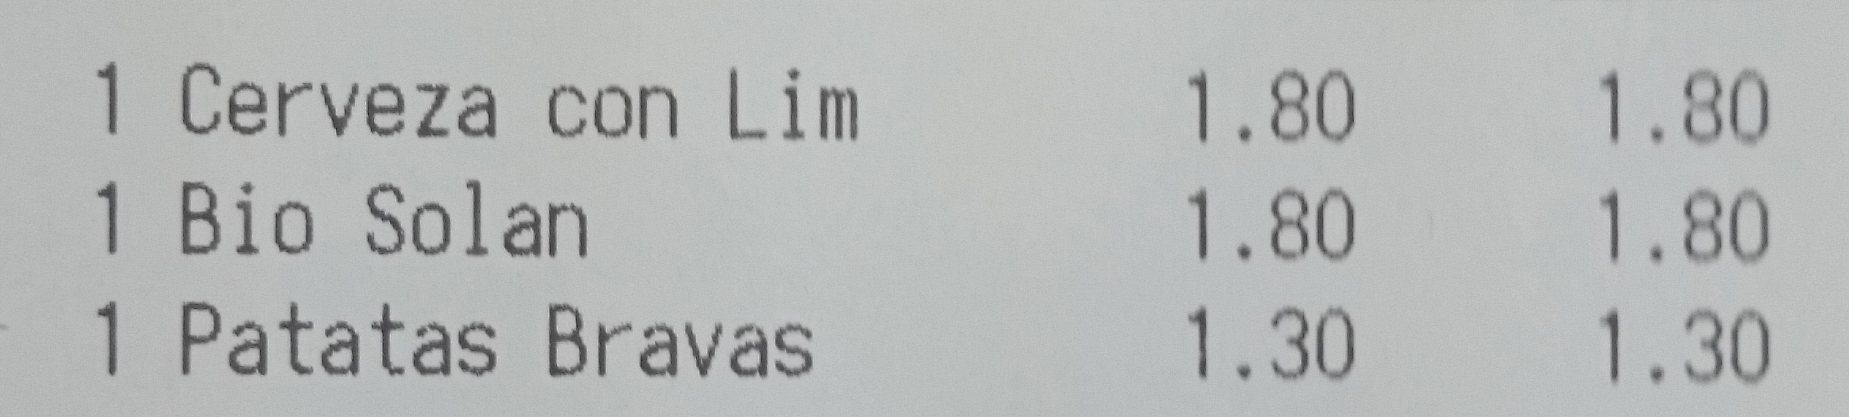
\includegraphics[width=\linewidth]{Recortada1.jpg}
		\caption{Recorte de la imagen original nº 1}
		\label{fig:recortada1}
		\end{minipage}
		\begin{minipage}[b]{0.45\linewidth}
			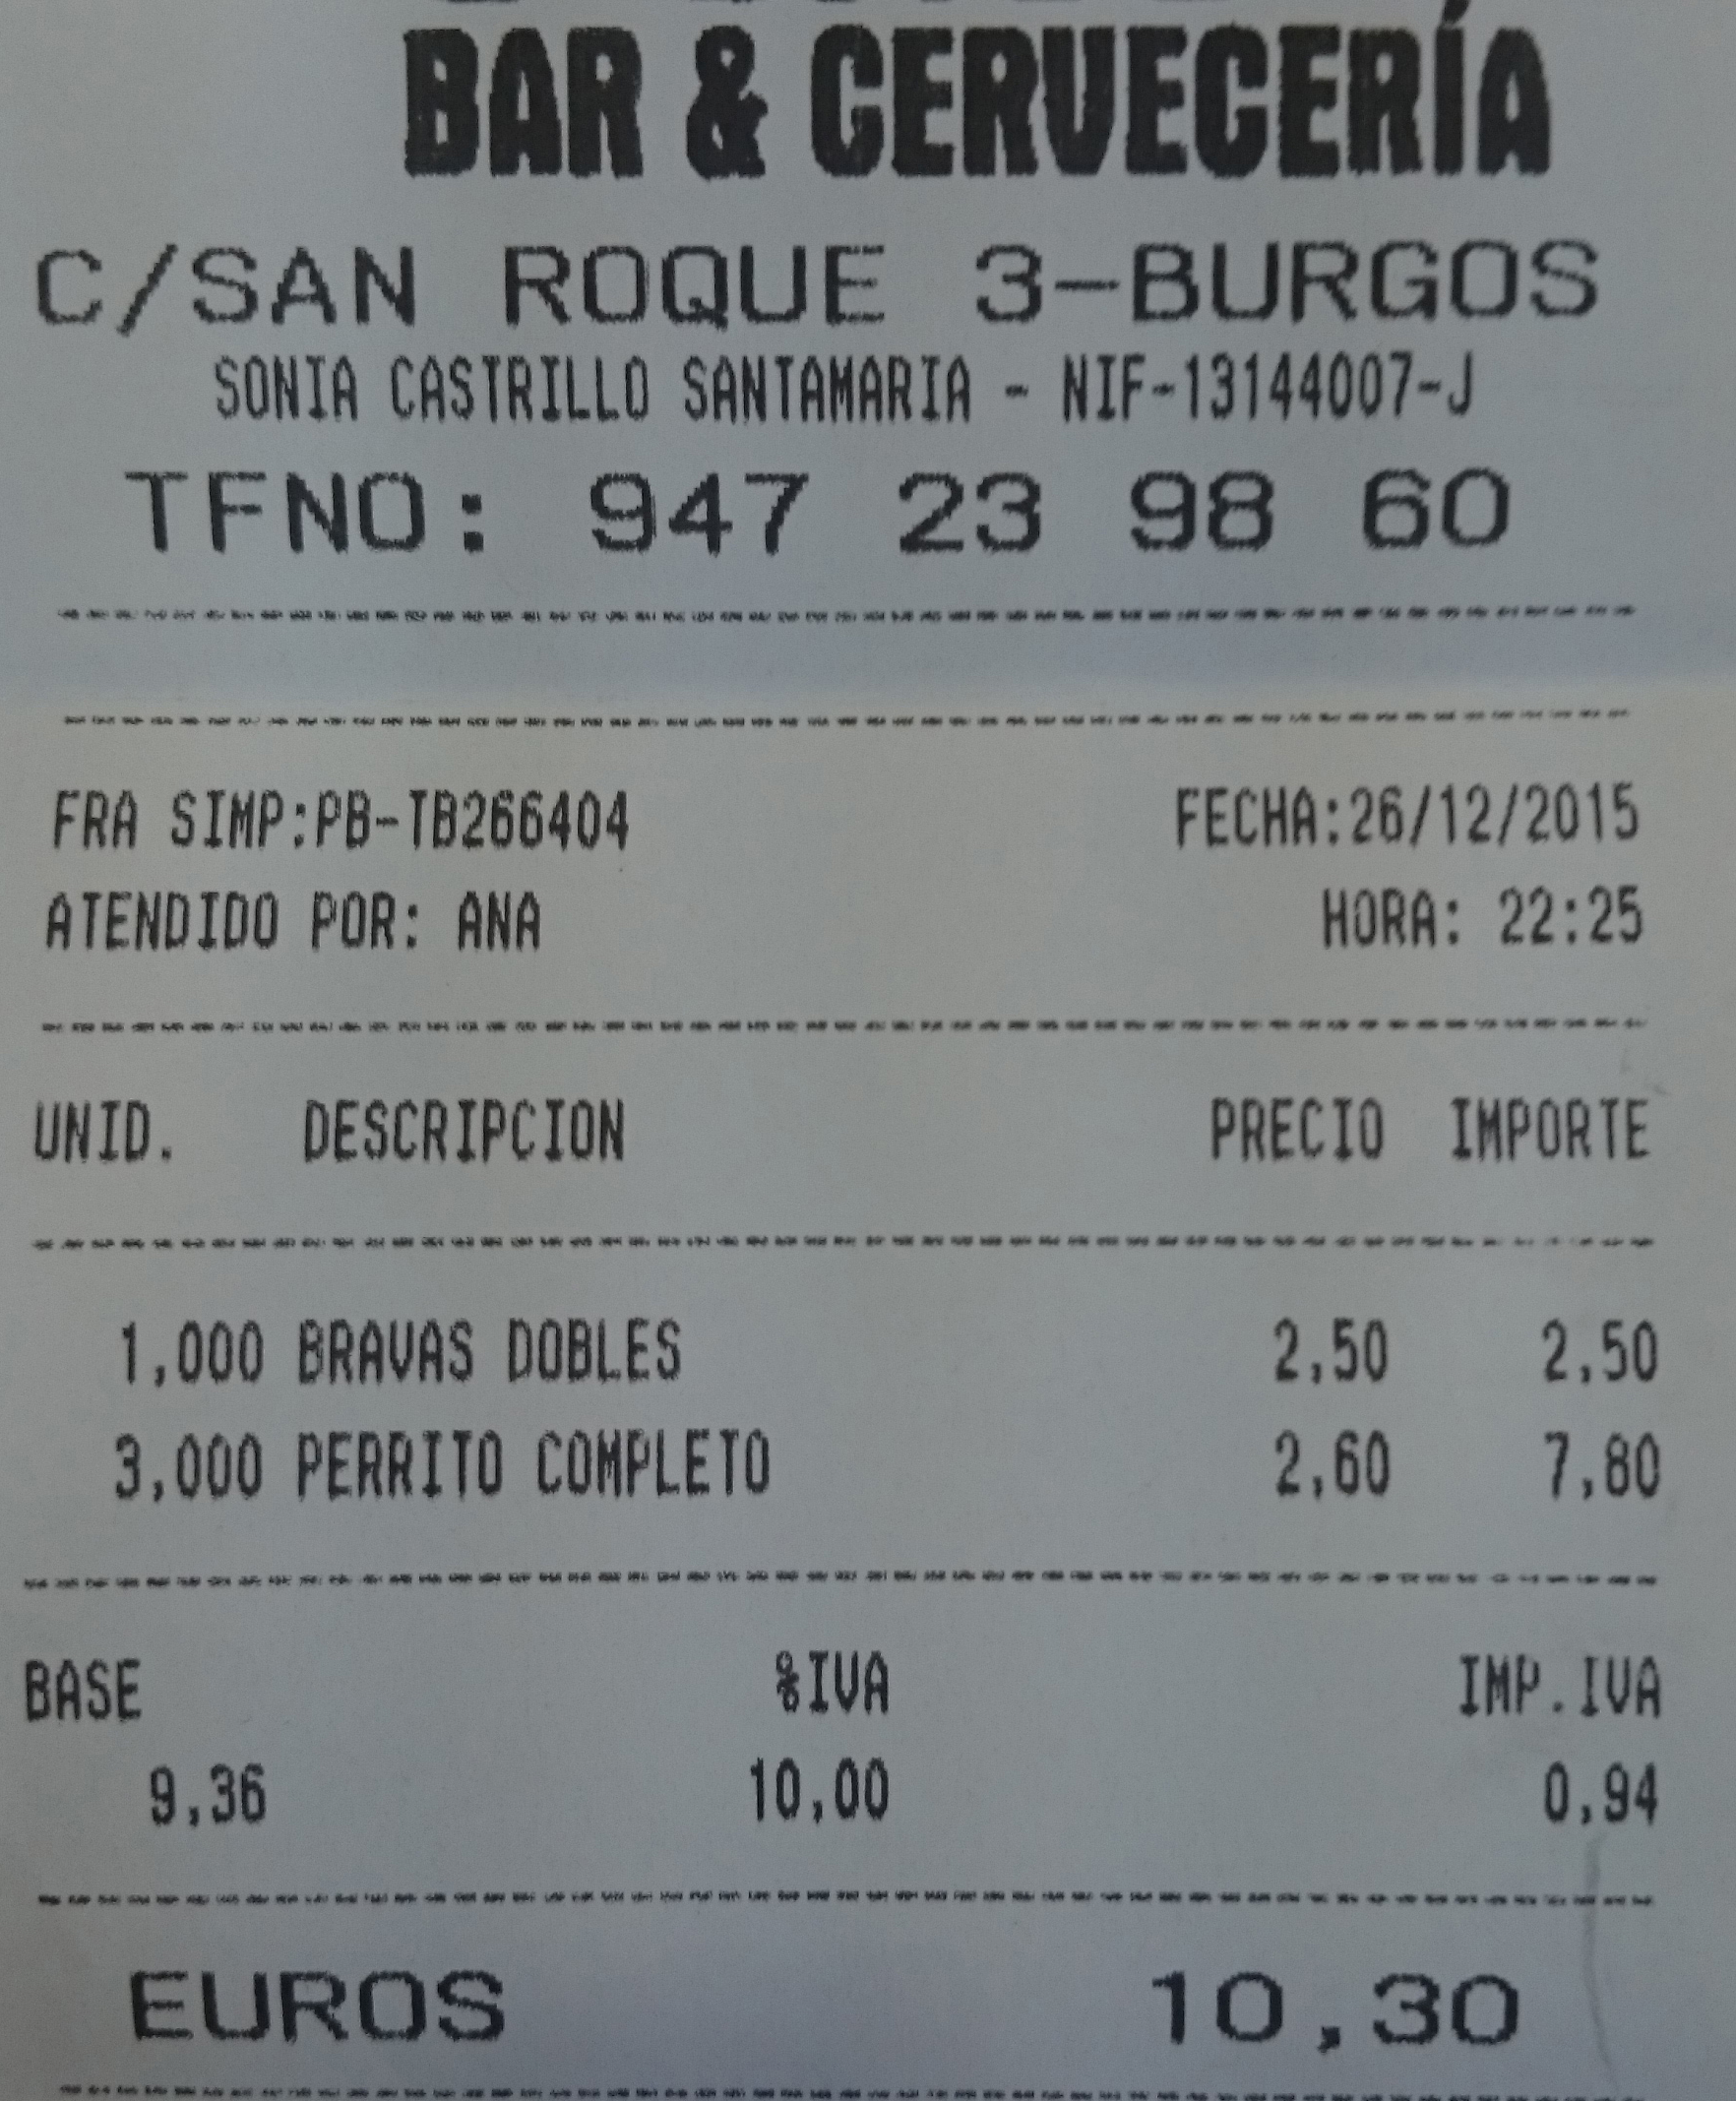
\includegraphics[width=\linewidth]{Original2.jpg}
			\caption{Imagen Original nº 2}
			\label{fig:original2}
	\end{minipage}
	\quad
	\begin{minipage}[b]{0.45\linewidth}
		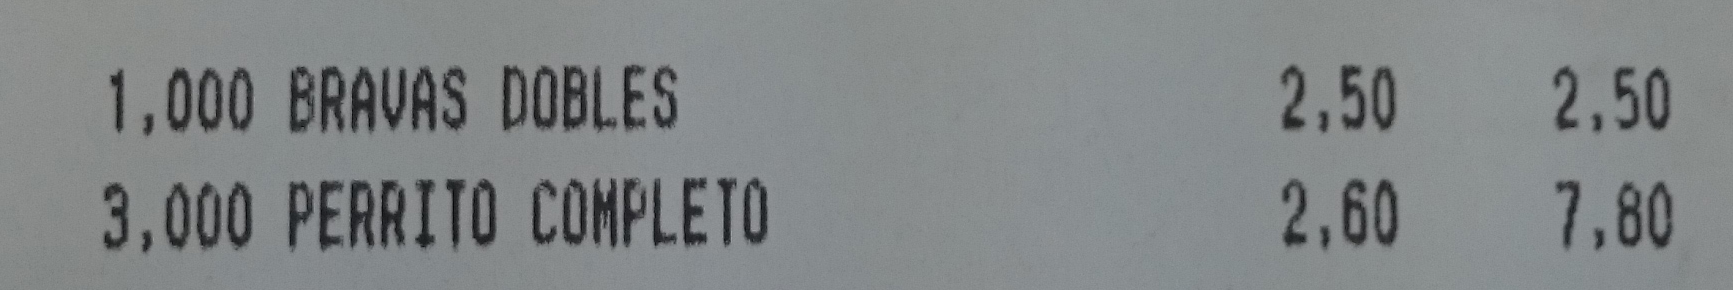
\includegraphics[width=\linewidth]{Recortada2.jpg}
		\caption{Recorte de la imagen original nº 2}
		\label{fig:recortada2}
		\end{minipage}
	\end{figure}
	


\clearpage

Estas pruebas han sido resumidas según el porcentaje de acierto (caracteres acertados / número total de caracteres) en las tablas \ref{tesseractingles} y \ref{tesseractespa}


\begin{table}[ht]
\rowcolors {2}{gray!35}{}
\center
\begin{tabular}{l c c c c}
\toprule
    Imagen    & Normal        & En bloque & En linea & Palabra\\
    \otoprule
Imagen 1     &  0\%   &  0\%     & 0\%   &  0\%\\
Recortada 1  &    61\%&   100\%   & 0\%  & 0\%\\
Imagen 2     &     0\%    &    0\%   &  0\%  &  0\%\\
Recortada 2      &    81\%&   81\%   & 0\%  & 0\%\\
\bottomrule 
\end{tabular}
\label{tesseractingles}
\caption{Pruebas precision Tesseract diccionario Inglés}
\end{table}

\begin{table}[ht]
\rowcolors {2}{gray!35}{}
\center
\begin{tabular}{l c c c c}
\toprule
    Imagen    & Normal        & En bloque & En linea & Palabra\\
    \otoprule
Imagen 1     &  0\%   &  0\%     & 0\%   &  0\%\\
Recortada 1  &    61\%&   100\%   & 0\%  & 0\%\\
Imagen 2     &     0\%    &    0\%   &  0\%  &  0\%\\
Recortada 2      &    70\%&   79\%   & 0\%  & 0\%\\
\bottomrule 
\end{tabular}
\label{tesseractespa}
\caption{Pruebas precision Tesseract diccionario Español}
\end{table}

Como se observa en las tablas anteriores, si la imagen es recortada, y utilizando el diccionario de caracteres ingleses, el porcentaje de precisión es mayor, por lo tanto se decidió continuar con esta configuración.

\section{Plataforma Android}

La aplicación se ha orientado para dispositivos móviles, dado que esta clase de operaciones de guardado y consulta de gastos son útiles en situaciones que necesitamos echar un vistazo rápido a nuestros gastos en cualquier lugar.

La elección de la plataforma Android, no ha sido trivial, ya que hoy en día Android es el S.O mas usado en smartphones en España y el mundo.
\imagen{cuotaAndroid}{Cuota de Android en España}

Como se ve en la imagen \ref{fig:cuotaAndroid} Android domina claramente el sector muy por encima de su principal rival IOs.

A partir de este punto se decide que versión de API se va a emplear para desarollar la aplicación. En este caso se ha optado por Android 5.0 Lollipop, debido a que es la 2º versión en uso por detrás de kitkat ver Figura \ref{fig:versionesAndroid} , sin embargo KitKat esta empezando a decaer frente a Lollipop	. \cite{versionesAndroid}

Otro motivo de peso es el uso de Material Desing como concepto de diseño en el desarrollo de aplicaciones, que es mucho mas sencillo su implementación en sistemas Lollipop.

\imagen{versionesAndroid}{Cuota de versiones Android Diciembre 2015}

\section{¿ En dispositivo o en la Nube ?}

Uno de los pasos clave a la hora de desarrollar este proyecto es la elección de realizar la traducción de imagen en el dispositivo o en un servidor.
Como se explica en el articulo \cite{localVScloud}, tanto la realización del proceso de OCR en el dispositivo o en un servidor tiene sus ventajas e inconvenientes.
Dado que en los requisitos se quería desarrollar un modelo cliente servidor, se ha optado por esta opción permitiendo el ahorro en el tamaño del paquete de la aplicación una vez desplegada en el móvil.

La centralización del proceso también supone una ventaja a la hora de controlar la transformación imagen a texto, dado que se emplea un diccionario alimentado por todos los clientes y no un diccionario por cliente, permitiendo así un crecimiento mucho mas rápido del vocabulario de este.

\section{Conexión cliente Servidor}
El canal de conexión entre el cliente y el servidor es una parte fundamental para poder llevar a cabo el proyecto.
En los primeros días de desarrollo, la conexión se realizaba mediante socket, los cuales transmitían de forma correcta la imagen al servidor, pero finalmente se realizo un servicio Rest, que tenia mucho mas sentido, dado que el servidor necesitaba dar una respuesta en la misma petición del cliente, y su implementación es mucho mas sencilla.

El uso de un servicio Rest permite su reutilización en mas sistemas, pudiendo exportar las funcionalidades del servidor a otras plataformas cliente.

\section{Librería de Procesado de Imágenes}
La elección de la librería para realizar todo el procesado de imagen en un principió fue ImageJ dado su simplicidad y que el tutor ya había trabajado con ella en proyectos anteriores, sin embargo dada la escasa documentación de esta librería, se ha empleado OpenCV con una comunidad de desarrollo y documentación muy superior y un rendimiento mayor, por lo que las técnicas de visión artificial   han resultado mas sencillas de implementar.

\section{Obtención de las lineas de producto}

Como se ha visto en la sección \ref{precisionTesseract}, al recortar todas las lineas de producto de la imagen principal, la precisión era mayour que si no se realizaba el recorte(ver tablas \ref{tesseractingles} y \ref{tesseractespa}), durante el tiempo que se trabajo en el presente trabajo, se desarrollo una forma de obtener una a una las lineas de producto de cada tique.Para ello una vez la imagen se en encuentra binarizada(ver sección \ref{ocr}), se realiza una dilatación que tiene como entrada la imagen binarizada y un operador morfológico en forma de recta (ver sección ) , con una altura de uno y un ancho igual al tamaño de la imagen que se esta analizando, lo que lleva a que el texto de las lineas de producto se transforme en rectángulos blancos como se puede ver en las imágenes.

\begin{figure}[ht]
		\centering
		\begin{minipage}[b]{0.45\linewidth}
			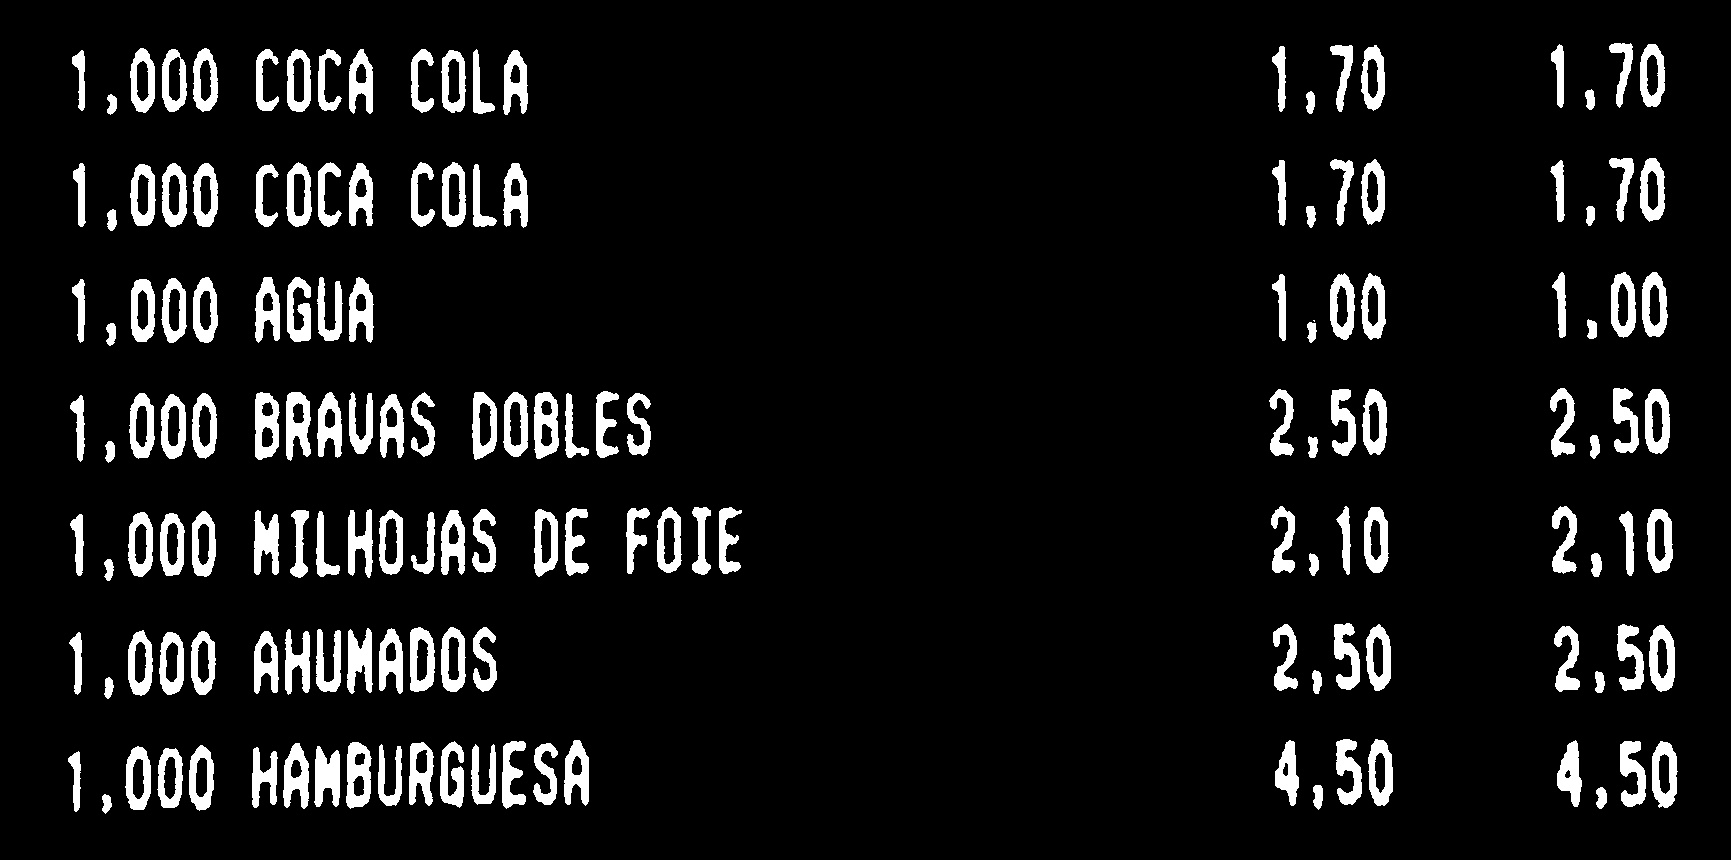
\includegraphics[width=\linewidth]{tiqueBinarizado.jpg}
			\caption{Imagen binarizada antes de dilatar}
			\label{fig:tiqueBinarizado}
	\end{minipage}
	\quad
	\begin{minipage}[b]{0.45\linewidth}
		
\includegraphics[width=\linewidth]{tiqueDilatado.jpg}
		\caption{Imagen dilatada donde se observan los rectángulos}
		\label{fig:tiqueDilatado}
		\end{minipage}
	\end{figure}

Cuando se obtienen estos rectángulos, es muy fácil conocer donde se entran las regiones que contienen las distintas lineas de productos, por ello se guarda cada linea de producto en un fichero de imagen distinto para poder después emplearlo como entrada en Tesseract.

\imagen{tiqueCortado}{Regiones de las distintas lineas de producto}

\section{Mejora de Tesseract}

Tesseract aplica por defecto su propio sistema para mejorar la imagen antes de realizar la conversión sin embargo, como se ve en \cite{improvequality}, si se aplica previamente  un algoritmo de deskewing puede mejorar la precision.

Dado que Tesseract suele cometer algún error a la hora de transformar imagen a texto, se ha desarrollado una forma de corregir las diferentes lineas de producto, para las descripción del producto se emplea  la distancia de Levenshtein(ver sección \ref{levenshtein}) aplicando un fichero de texto como soporte, es decir un diccionario, con esto se devuelve la palabra con la menor distancia, y con ello la mas parecida.

Dado que a los números de las lineas de producto no puede aplicarse una formula para corregirlos, se ha creado un fichero de concordancias por la forma del carácter que Tesseract interpreta por un número, esto se puede ver en el siguiente ejemplo:

\begin{center}
\textit{LOO REFRESCOS DE COLA 1.20 l.2U}
\end{center}

La cantidad y el importe total del la linea anterior está formada por letras y números.

\begin{table}[ht]
\rowcolors {2}{gray!35}{}
\center
\begin{tabular}{l c c c c}
\toprule
    Carácter    & Numero    \\
    \otoprule
	L 	&	1.\\
	l 	&	1\\
	O	&	0\\
	U	&	0\\
\bottomrule 
\end{tabular}
\label{tablaCsv}
\caption{Extracto del fichero de correspondencias}
\end{table}

Si aplicamos el fichero de correspondencias, podemos ver un extracto en la tabla \ref{tablaCsv}, la corrección resultante es:

\begin{center}
\textit{1.00 REFRESCOS DE COLA 1.20 1.20}
\end{center}
Con estas 2 medidas se consigue una gran mejora en las conversiones.

